% Results section for the H1 high-Q^2 charged-particle SIDIS analysis note.
\section{Results}
\label{sec:results}

\begin{tcolorbox}[colback=yellow!8,colframe=orange!70,title={\bfseries Current release status}]
The current nominal central-value chain is the 2026-10-20 OPT-A baseline
promotion, in which the response truth contract is harmonized to the
radiative correction (Sec.~\ref{sec:unfolding:truth-contract}).  Its
reconstructed-level definition combines the $\alpha\ge0.2~\mathrm{rad}$
laboratory-frame scattered-electron cone with the
detector-interaction-corrected response, and the electron, V0, and
low-$\Qsq$ background templates are subtracted from the data vector before
unfolding.  The cross section is Born-level provisional:
$C_{\mathrm{rad}}$ is applied per-bin post-unfold from the DJANGOH14 table
binned as the release, with its uncertainty carried as the radiative
generator-difference and radiative-statistics components.  The
$E-p_z>45~\GeV$ convention is retained.  The systematic budget is being
regenerated on this nominal: the frozen budget editions on file were
computed on the superseded central values, are superseded as a quoting
basis, and no per-bin uncertainty or uncertainty total is final until the
regenerated budget passes review
(Sec.~\ref{sec:syst:budget-regeneration}).  The 2026-10-17 clean release
and the 2026-10-15 Born release are superseded for the nominal and retained
untouched as provenance.  The exposure of the simulated
radiative samples is reconciled file by file, but the generator-log
cross-check is permanently blocked externally, so the radiative correction
remains provisional and the release is not publication-grade.  The
$C_{\mathrm{rad}}$ multiplicity mapping and the
corrected inclusive DIS denominator are still pending.  Numerical
multiplicities and final physics tables should therefore be regarded as
preliminary until the denominator is available.
\end{tcolorbox}

\subsection{Working Release}
\label{sec:results:z005-release}

The current high-$\Qsq$ working release contains 490 published bins in total,
with 245 $\hplus$ rows and 245 $\hminus$ rows.  The nominal unfolding method is
iterative Bayesian unfolding with four selected iterations.  The data vector
length is 980, and the per-charge response shape is $(491,246)$.

The canonical raw release is
\path{bbb_ibu_bgsub_setRprime_conebase_optA_q2esgen_S3xmerged_zlow005_pT5_eta1p6_radlen5_nhit5_2026-10-20/}
under \path{H1ChargedSidis_HighQ2/output_v6/central/data_release/}, and its
Born-level product is the in-tree \path{born_crad_applied/} directory of the
same release.  Both use the response matrix's own generator-level
distribution as the unfolding prior, on the harmonized response of
Sec.~\ref{sec:unfolding:truth-contract}.  Integrated over the 490 published
bins at $\mathcal{L}_{\mathrm{data}}=351000.0~\mathrm{nb}^{-1}$, the raw
release gives IBU $10.511329~\mathrm{nb}$ ($\hplus$) and
$10.219863~\mathrm{nb}$ ($\hminus$); the Born-level product gives IBU
$11.997446~\mathrm{nb}$ ($\hplus$) and $11.664706~\mathrm{nb}$
($\hminus$).

This release supersedes for the nominal the 2026-10-17 clean release
\path{bbb_ibu_bgsub_setRprime_conebase_S3xmerged_zlow005_pT5_eta1p6_radlen5_nhit5_2026-10-17/}
and its 2026-10-15 Born parent
\path{born_crad_bgsub_setRprime_conebase_S3xmerged_zlow005_pT5_eta1p6_radlen5_nhit5_2026-10-15/},
which are retained untouched as provenance; their integrated values
($10.508811~\mathrm{nb}$ and $10.217503~\mathrm{nb}$ raw,
$11.996558~\mathrm{nb}$ and $11.663956~\mathrm{nb}$ Born) are superseded
central values.  The promotion moves the integrated raw totals by $+0.0240\%$
($\hplus$) and $+0.0231\%$ ($\hminus$) and the Born totals by $+0.0074\%$ and
$+0.0064\%$.  Per cell, the Born shifts have absolute medians of $1.05\%$
($\hplus$) and $1.15\%$ ($\hminus$), and the largest populated shift is
$+4.2051\%$ (negative charge, global bin 159), below its full-sample net
straddle rate of $+4.9191\%$ (ratio $0.855$); every well-populated per-cell
shift is bounded by its full-sample per-cell straddle rate, the complete
exception set being the adjudicated 48-cell list of
Sec.~\ref{sec:unfolding:truth-contract}.  The change is a
one-time central-value correction---the removal of the response binning bias
documented in Sec.~\ref{sec:unfolding:truth-contract}---and is not carried
as an uncertainty.  The background
subtraction removes $281{,}250.09$ tracks, $7.2767\%$, from the cone data
vector of $3{,}865{,}073$ in-grid entries before the unfolding:
$148{,}976.4$ electron and positron tracks, $132{,}065.3$ V0 decay daughters,
and $208.4$ low-$\Qsq$ leakage tracks.  The subtracted data vector itself is
unchanged by the promotion.  The detector-interaction class is not
part of this external subtraction: it is removed response-internally through
the per-reco-bin fake fraction $f_i$ of the detector-interaction-corrected
response, and an external subtraction of it would double-remove the class.
For lineage, the immediately preceding release with the electron cone but no
background subtraction, which unfolds the full cone data vector, integrates to
raw IBU
values of $11.412233~\mathrm{nb}$ ($\hplus$) and $11.123626~\mathrm{nb}$
($\hminus$); these superseded values are retained only as the historical
parent of the current release and are not current results.

The systematic budget is being regenerated on this nominal
(Sec.~\ref{sec:syst:budget-regeneration}).  The most recent frozen editions,
the twenty-active-term 2026-10-19 edition and its nineteen-component
2026-10-17 parent, were computed on the superseded central values; they are
superseded as a quoting basis and retained unchanged as provenance, and the
per-bin uncertainties and totals of those editions must not be quoted as
final until the regenerated budget passes review.  The component inventory
of those editions is described in
Sec.~\ref{sec:systematics}.

The central IBU implementation has an independent numerical cross-check:
RooUnfoldBayes reproduces the in-house iterative-Bayesian yields to a maximum
relative precision of $2.6\times10^{-15}$ across 980 rows.  This comparison
covers both RAPGAP and DJANGOH response inputs and has no invalid or
zero-denominator bins.

\subsection{Diagnostic Four-Dimensional Cross-Section Plots}
\label{sec:results:diagnostic-4d-cross-sections}

The plotted observable used for diagnostic data--MC comparisons is the
four-dimensional differential cross section,
\begin{equation}
  \frac{\mathrm{d}^{4}\sigma}{\mathrm{d}\Qsq\,\mathrm{d}x\,
  \mathrm{d}z\,\mathrm{d}\pTh}
  = \frac{\sigma_{\mathrm{bin}}}{\Delta\Qsq\,\Delta x\,\Delta z\,\Delta\pTh},
  \label{eq:results:four-dimensional-cross-section-density}
\end{equation}
in units of $\mathrm{nb}\,\GeV^{-3}$, since the $\mathrm{d}\Qsq$ differential
contributes $\GeV^{2}$. For the capped top-$x$ cell, $\Delta x=1.0-x_{\min}$.

The current five-prediction comparison package is
\path{plots/mc_predictions/data_vs_mc_z005_5generator_born_releasebin_2026-10-13/}.
Its data side is the superseded raw release without the electron cone,
corrected to the photon-Born level without the $Z$-exchange contribution.  It is a DJANGOH-only provisional diagnostic: the
four generator curves are at full-Born/NORAD level while the data side is
photon-Born, producing a known level difference of about $9\%$ by design;
only MAPTMD24 is photon-only.  The package has not been regenerated on the
current cone-based observable basis and its figures are not referenced in this
note.  MAPTMD24 covers 230 of 490 published bins, with no $z<0.05$ row and
sparse $\pTh$ coverage at higher $z$; this is the final limitation of that
comparison.  The package remains a PROVISIONAL INTERNAL DIAGNOSTIC.

\subsection{Diagnostic Cross-Section Density with the Near-Electron Veto}
\label{sec:results:diagnostic-alpha0p2-cross-section-density}

Figures~\ref{fig:results:alpha0p2-xsec-density-hplus} and
\ref{fig:results:alpha0p2-xsec-density-hminus} show the IBU-only
cross-section-density diagnostic for the near-electron opening-angle veto,
which rejects tracks with $\alpha<0.2$.  The plotted observable is the
four-dimensional differential cross section defined in
Eq.~\ref{eq:results:four-dimensional-cross-section-density}, using the same 4D
bin-volume normalization.  The input is the rescaled IBU release CSV from this
study, with $\mathcal{L}_{\mathrm{data}}=351~\pbinv$, the selection
$|\eta|<1.6$, radial track length at least $5~\mathrm{cm}$, and at least five
CJC hits, and the measurement binning.

The seven displayed $(\Qsq,x)$ intervals are listed in
Table~\ref{tab:binning:z005-contract}. Each charge plot contains these seven
cells, seven $z$ bins, and five $\pTh$ bins, for 490 plotted points in total
across both charges and no skipped bins. All densities use the physical cap
$\Delta x=1.0-x_{\min}$; the figures in this section were regenerated on
2026-10-16 with this convention.
The horizontal uncertainty is the $\pTh$ half-bin width.  The vertical
uncertainty is the quadrature sum of the statistical, model, and
regularization uncertainties, divided by the 4D bin volume; no additional
systematic components are included in these error bars.

The plots are retained here as diagnostic/provisional products only: they are
raw pre-Born inputs from an earlier, superseded release lineage, without
background subtraction or $C_{\mathrm{rad}}$.
Final approval remains pending; the plots are not for public release or
citation, and multiplicities remain blocked because no corrected inclusive DIS
denominator is available. For the cross section the radiative correction is no
longer pending: $C_{\mathrm{rad}}$ is applied per-bin post-unfold in the
current Born-level provisional release, with its uncertainty carried as the
radiative generator-difference and radiative-statistics components;
these selection-variant plots have not been regenerated on the current,
background-subtracted release.  Final release remains blocked by
publication-grade clearance of the radiative correction and by the
registration of the final publication plotting and systematics-rendering
chain.

\begin{figure}[p]
  \centering
  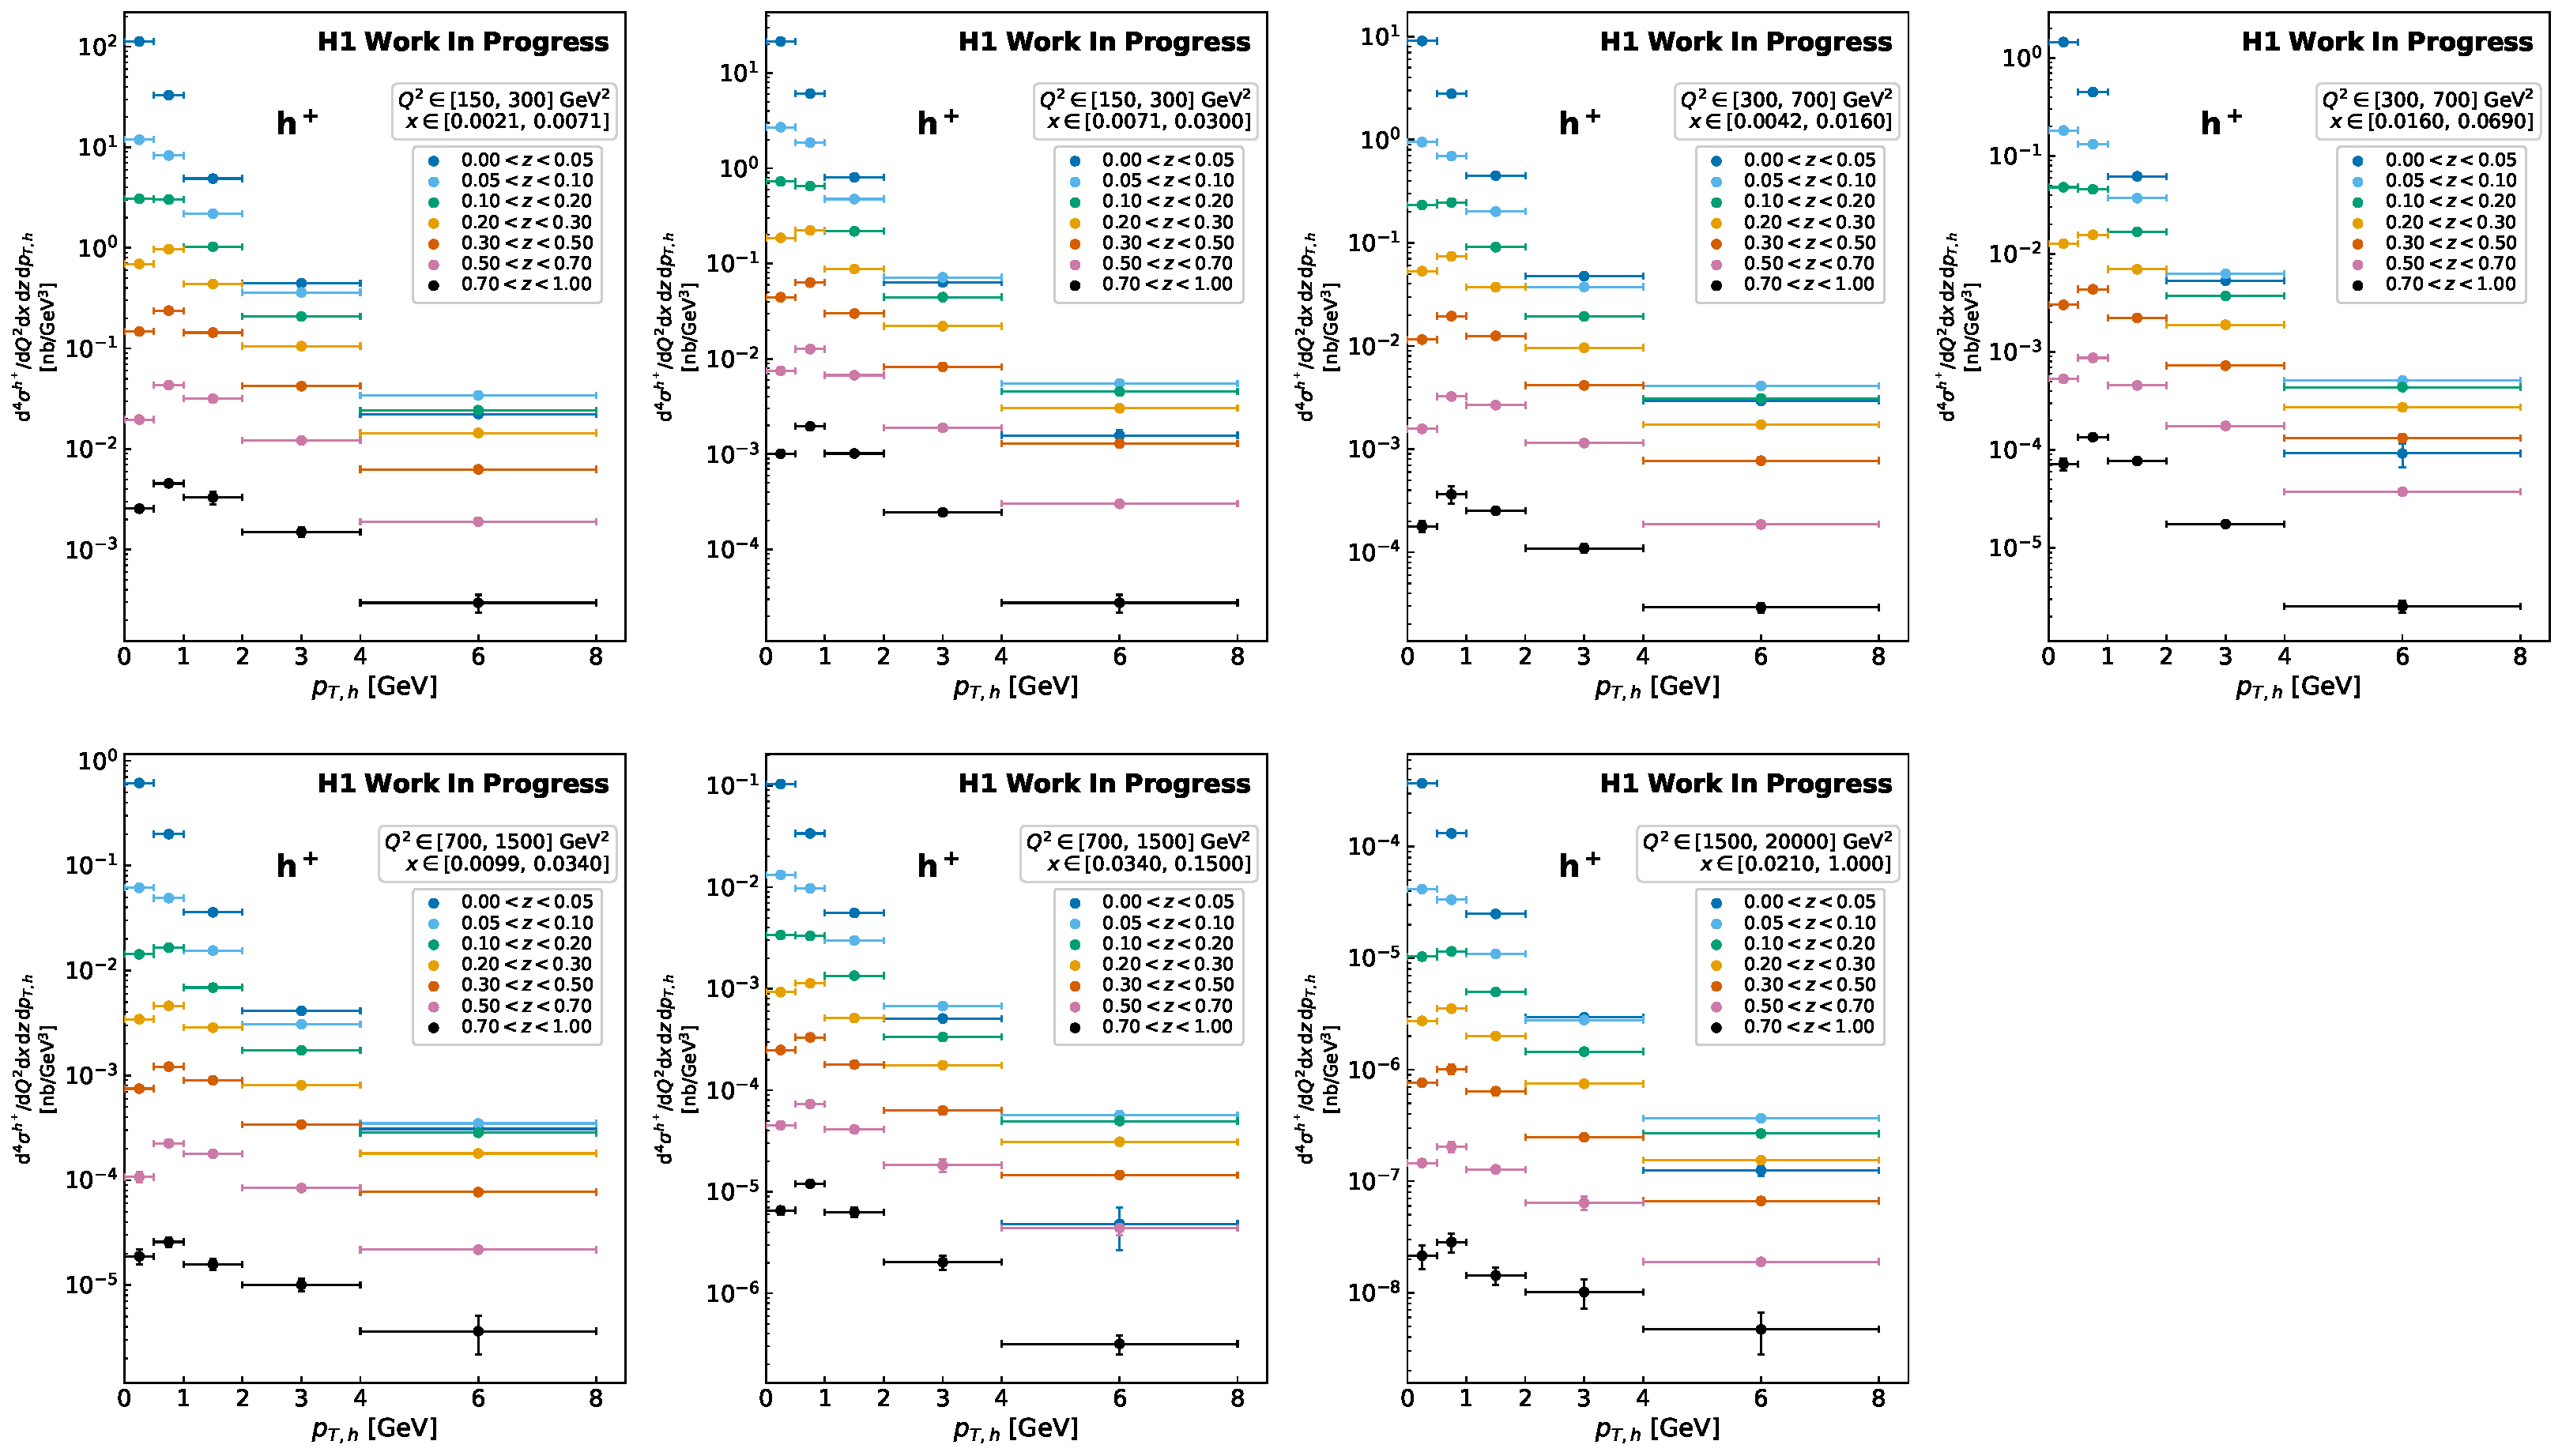
\includegraphics[width=0.98\textwidth,height=0.82\textheight,keepaspectratio]{figures/fig_results_xsec_density_alpha0p2_7panel_hplus_z005.pdf}
  \caption{Diagnostic/provisional cross-section density with the near-electron
  opening-angle veto for $\hplus$, plotted as
  $\mathrm{d}^{4}\sigma/(\mathrm{d}\Qsq\,\mathrm{d}x\,
  \mathrm{d}z\,\mathrm{d}\pTh)$ in $\mathrm{nb}\,\GeV^{-3}$.  The nominal
  iterative Bayesian unfolding is shown for $351~\pbinv$ in seven $(\Qsq,x)$ cells, seven $z$ bins,
  and five $\pTh$ bins.  Vertical uncertainties combine the statistical,
  model, and regularization contributions in quadrature and are divided by the
  4D bin volume; horizontal uncertainties are $\pTh$ half-bin widths.  No
  additional systematic components are included.  This raw pre-Born diagnostic
  is a superseded historical render with no background subtraction or
  $C_{\mathrm{rad}}$ correction, predating the current release, which applies
  both a pre-unfold background subtraction and the per-bin post-unfold
  $C_{\mathrm{rad}}$ correction; it is not for public release or citation.}
  \label{fig:results:alpha0p2-xsec-density-hplus}
\end{figure}

\begin{figure}[p]
  \centering
  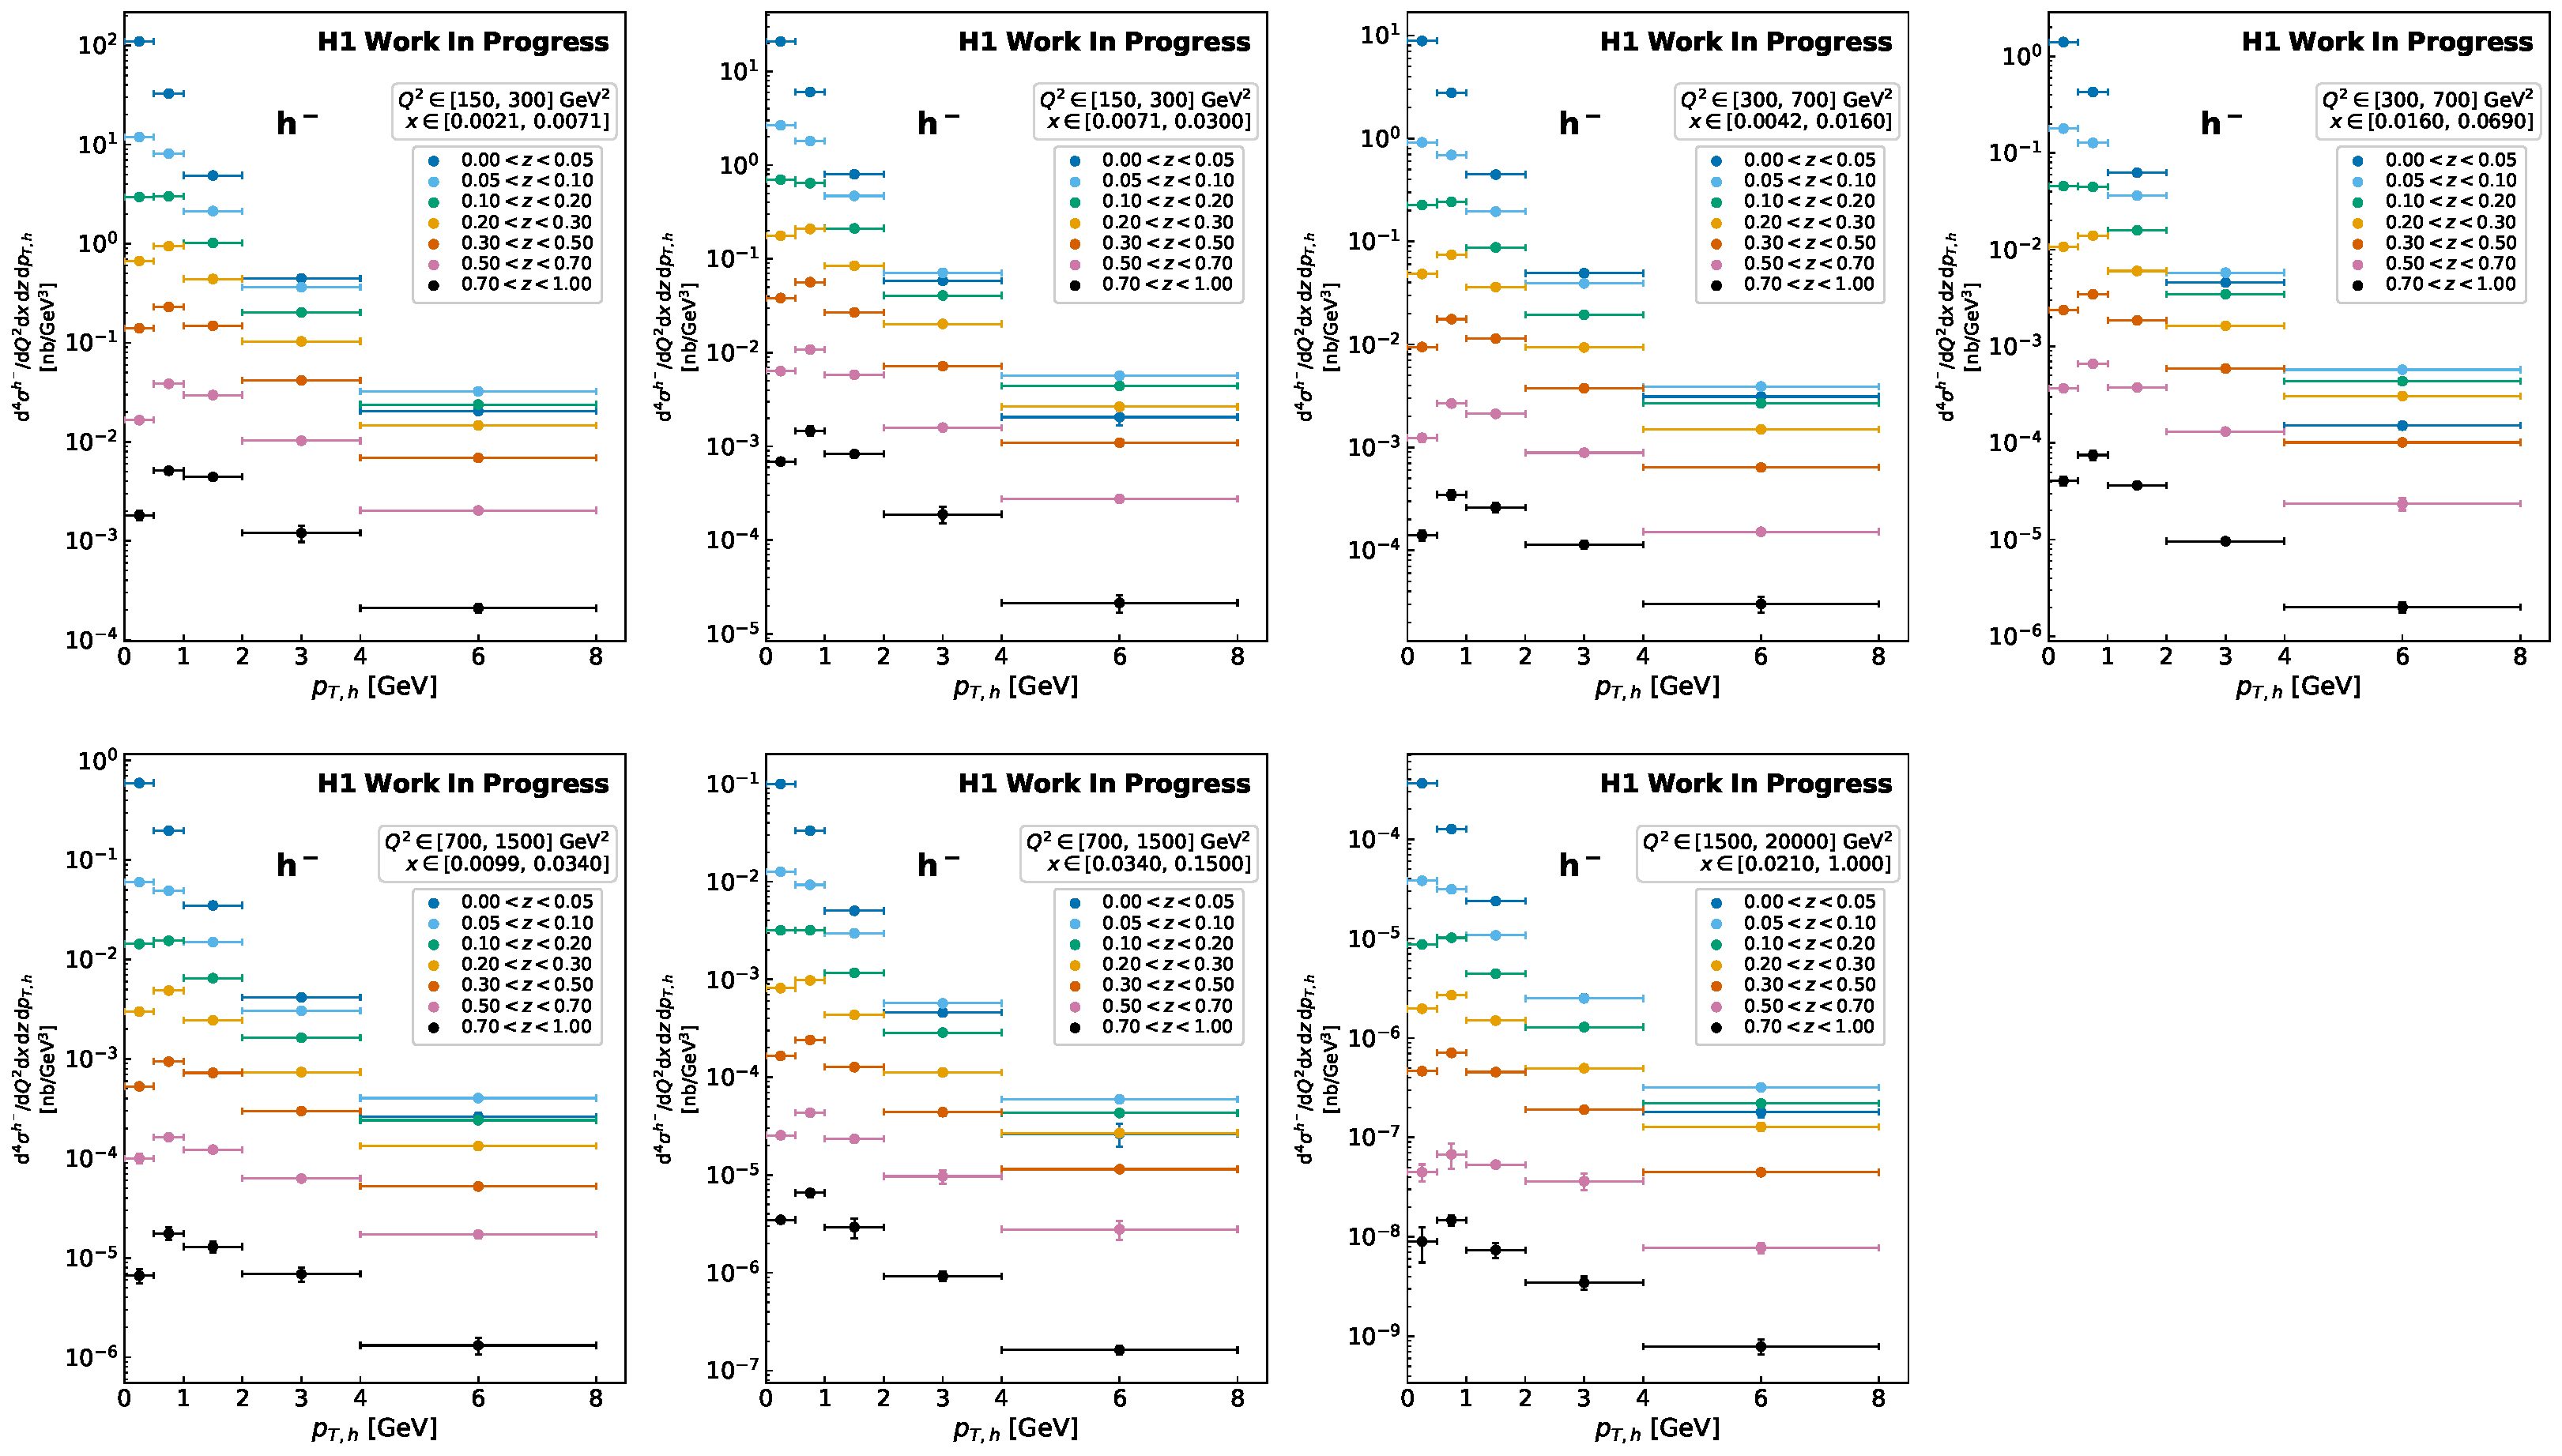
\includegraphics[width=0.98\textwidth,height=0.82\textheight,keepaspectratio]{figures/fig_results_xsec_density_alpha0p2_7panel_hminus_z005.pdf}
  \caption{Diagnostic/provisional cross-section density with the near-electron
  opening-angle veto for $\hminus$, plotted as
  $\mathrm{d}^{4}\sigma/(\mathrm{d}\Qsq\,\mathrm{d}x\,
  \mathrm{d}z\,\mathrm{d}\pTh)$ in $\mathrm{nb}\,\GeV^{-3}$.  The nominal
  iterative Bayesian unfolding is shown for $351~\pbinv$ in seven $(\Qsq,x)$ cells, seven $z$ bins,
  and five $\pTh$ bins.  Vertical uncertainties combine the statistical,
  model, and regularization contributions in quadrature and are divided by the
  4D bin volume; horizontal uncertainties are $\pTh$ half-bin widths.  No
  additional systematic components are included.  This raw pre-Born diagnostic
  is a superseded historical render with no background subtraction or
  $C_{\mathrm{rad}}$ correction, predating the current release, which applies
  both a pre-unfold background subtraction and the per-bin post-unfold
  $C_{\mathrm{rad}}$ correction; it is not for public release or citation.}
  \label{fig:results:alpha0p2-xsec-density-hminus}
\end{figure}

\subsection{Born-Level Provisional Cross-Section Density}
\label{sec:results:release351-expanded-xsec-density}

Figures~\ref{fig:results:release351-cone-xsec-density-hplus}
and~\ref{fig:results:release351-cone-xsec-density-hminus} show the Born-level
provisional cross-section densities of the background-subtracted
clean-release chain, obtained with the iterative Bayesian unfolding and the
response matrix's own generator-level prior.  The observable is
defined in Eq.~\ref{eq:results:four-dimensional-cross-section-density}.
These renders predate the 2026-10-20 OPT-A baseline promotion: their input is
the Born-level release
\path{born_crad_bgsub_setRprime_conebase_S3xmerged_zlow005_pT5_eta1p6_radlen5_nhit5_2026-10-15/}
under \path{H1ChargedSidis_HighQ2/output_v6/central/data_release/}, at
$\mathcal{L}_{\mathrm{data}}=351000.0~\mathrm{nb}^{-1}$, whose integrated IBU
totals, $11.996558~\mathrm{nb}$ for $\hplus$ and $11.663956~\mathrm{nb}$ for
$\hminus$ over the 490 published bins, are superseded central values
(Sec.~\ref{sec:results:z005-release}); the figures are retained until the
canonical plotting chain is re-pointed to the OPT-A nominal and the
regenerated budget is available.  $C_{\mathrm{rad}}$ is applied
per-bin post-unfold from the DJANGOH14 (xFGen$<$0, EMPZ$>$45) table, whose
integrated factors are 1.142 for $\hplus$ and 1.141 for $\hminus$; the
EMPZ$>$45 convention is retained.  The plotted points are the
background-subtracted Born-level values: the electron, V0, and low-$\Qsq$
backgrounds are subtracted from the data vector before unfolding, and the
detector-interaction class is removed response-internally through the
per-reco-bin fake fraction $f_i$.  Each charge plot contains seven
$(\Qsq,x)$ cells, seven $z$ bins, and five $\pTh$ bins, for 490 points across
both charges.

The vertical uncertainty bands show the quoted total systematic uncertainty of
the frozen 2026-10-19 budget, including the two radiative components.  This
budget combines twenty active quadrature terms on the background-subtracted
basis; its median totals are $7.320288331169215\%$ for $\hplus$ and
$7.637124635311324\%$ for $\hminus$, and no bin exceeds $100\%$.  The frozen
editions were computed on the superseded central values and are superseded as
a quoting basis, so these bands are not final: no per-bin uncertainty or
total is final until the budget regenerated on the OPT-A nominal passes
review (Sec.~\ref{sec:syst:budget-regeneration}).  These are not final
central values: the release is Born-level provisional, not physics-final,
and the figures carry internal-review status only.

Two plot packages document the OPT-A promotion itself; both were accepted on
visual review and neither carries final uncertainties.  The user-facing
new-versus-old comparison set (nine pages) is
\path{H1ChargedSidis_HighQ2/output_v6/studies/optA_response_rebuild_2026-10-19/plots/comparison_newvsold_2026-10-20/}:
integrated raw and Born new-versus-old bars, per-cell raw-difference panels
with the straddle overlay, logarithmic old-versus-new scatters with the 48
flagged cells and the corner bins b39, b109, and b179 marked,
shift-versus-straddle bound scatters, and signed per-cell shift maps.  The
publication-facing canonical category-7 package is
\path{plots/canonical_2026-10-20_opta/} inside the OPT-A release tree of
Sec.~\ref{sec:results:z005-release}: four PDFs of the background-subtracted
OPT-A nominal, with the Born level obtained from the unchanged DJANGOH14
table and the uncertainty bands omitted pending the budget regeneration.  The
remaining canonical categories are pending the same regeneration
(Sec.~\ref{sec:syst:budget-regeneration}).

For lineage, Figures~\ref{fig:results:release351-expanded-xsec-density-hplus}
and~\ref{fig:results:release351-expanded-xsec-density-hminus} retain the
previous Born-level rendering of the same observable from the superseded
xFcut basis, which predates the detector-interaction correction.  Their input
is the Born release
\path{born_crad_dj14xfcut_S3xmerged_zlow005_pT5_eta1p6_radlen5_nhit5_2026-10-07/}
under \path{H1ChargedSidis_HighQ2/output_v6/central/data_release/}, at
$\mathcal{L}_{\mathrm{data}}=351000.0~\mathrm{nb}^{-1}$; the corresponding
raw pre-$C_{\mathrm{rad}}$ release, the coherent-prior raw parent of that
Born release, integrates to 22.67~nb over the 490 bins.
$C_{\mathrm{rad}}$ is applied per-bin post-unfold from the DJANGOH14 xFcut
(xFGen$<$0, EMPZ$>$45) table, whose integrated factors are 1.142 for
$\hplus$ and 1.141 for $\hminus$.  The vertical error bars show the full
13-component systematic total of the superseded budget
\texttt{total\_uncertainty\_z005\_coherentprior\_b1floor\_crad13\_2026-10-07/}
under \texttt{H1ChargedSidis\_HighQ2/output\_v6/systematics/summary\_plots/},
with median totals of 5.713\% for $\hplus$ and 6.150\% for $\hminus$.  These
values predate the detector-interaction correction and the cone baseline: those
promotions changed the observable basis, so the two figure sets must not be
compared bin by bin.

\begin{figure}[p]
  \centering
  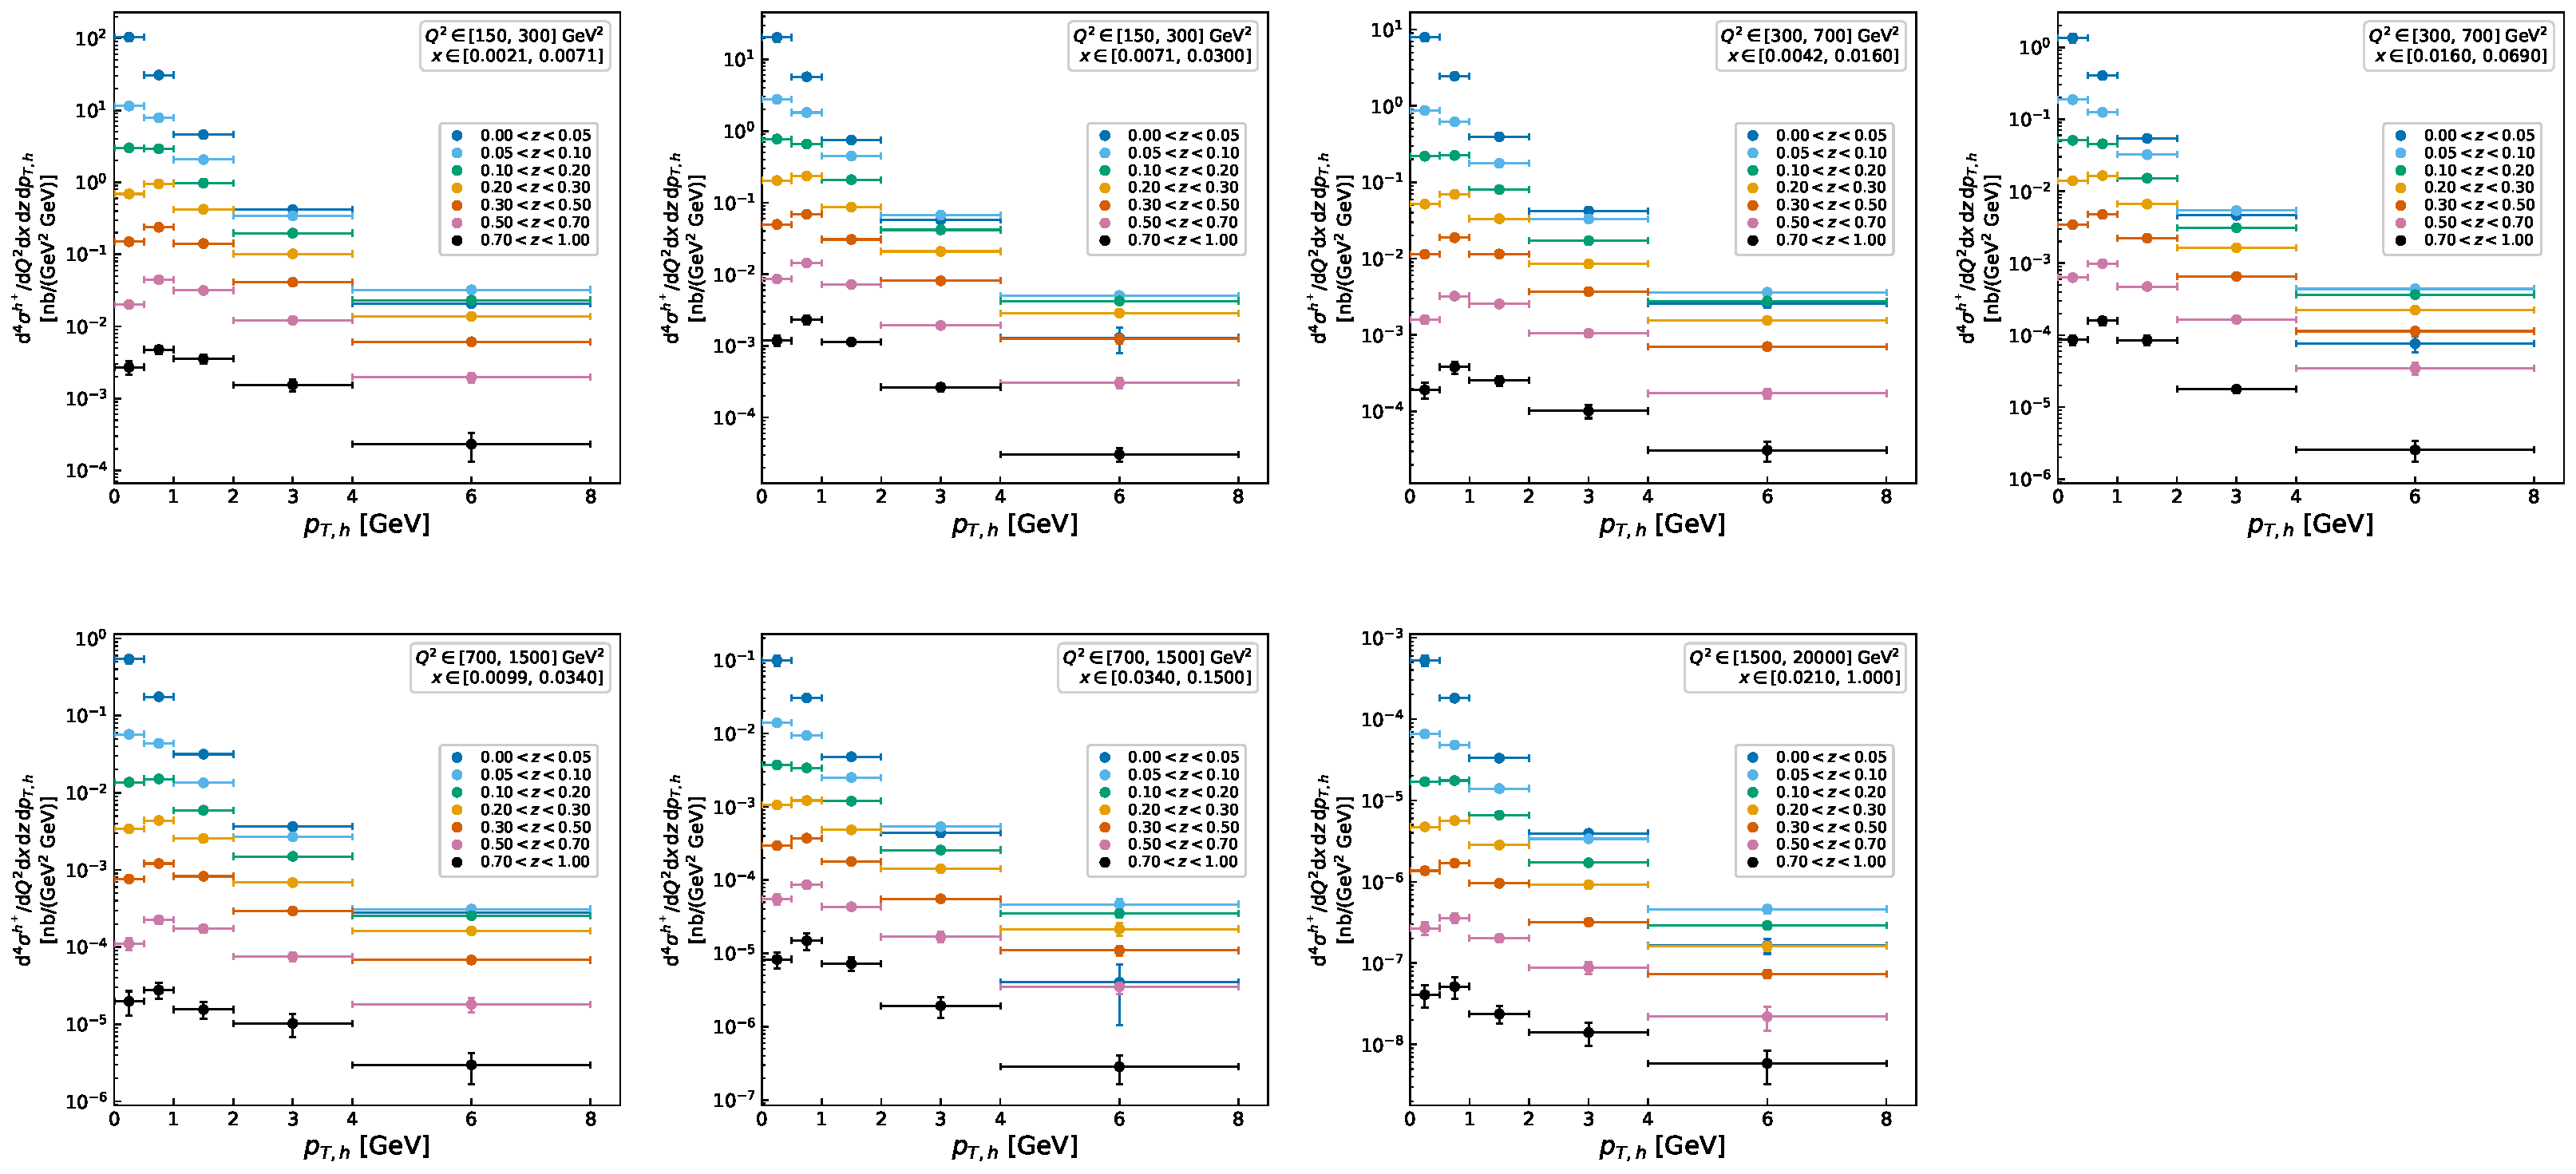
\includegraphics[width=0.98\textwidth,height=0.82\textheight,keepaspectratio]{figures/fig_results_xsec_density_born_cone_env100_7panel_hplus_z005_20261019.pdf}
  \caption{Born-level provisional cross-section density for $\hplus$
  from the iterative Bayesian unfolding, plotted as
  $\mathrm{d}^{4}\sigma/(\mathrm{d}\Qsq\,\mathrm{d}x\,
  \mathrm{d}z\,\mathrm{d}\pTh)$ in $\mathrm{nb}\,\GeV^{-3}$, at
  $\mathcal{L}_{\mathrm{data}}=351000.0~\mathrm{nb}^{-1}$.
  $C_{\mathrm{rad}}$ is applied per-bin post-unfold from the DJANGOH14
  (xFGen$<$0, EMPZ$>$45) table.  The points are the background-subtracted
  Born-level values of the superseded 2026-10-15 clean-release basis, which
  predates the OPT-A baseline promotion: the electron, V0, and low-$\Qsq$
  backgrounds are subtracted from the data vector before unfolding.  The band
  shows the quoted total systematic uncertainty of the frozen 2026-10-19
  budget, superseded as a quoting basis, whose median totals are
  $7.320288331169215\%$ for $\hplus$ and
  $7.637124635311324\%$ for $\hminus$.  This Born-level provisional figure
  carries internal-review status and is not physics-final.  Produced from the
  dated 2026-10-19 cross-section package
  \texttt{plots/cross\_sections/cone\_born\_7panel\_env100\_xcap\_2026-10-19/}.}
  \label{fig:results:release351-cone-xsec-density-hplus}
\end{figure}

\begin{figure}[p]
  \centering
  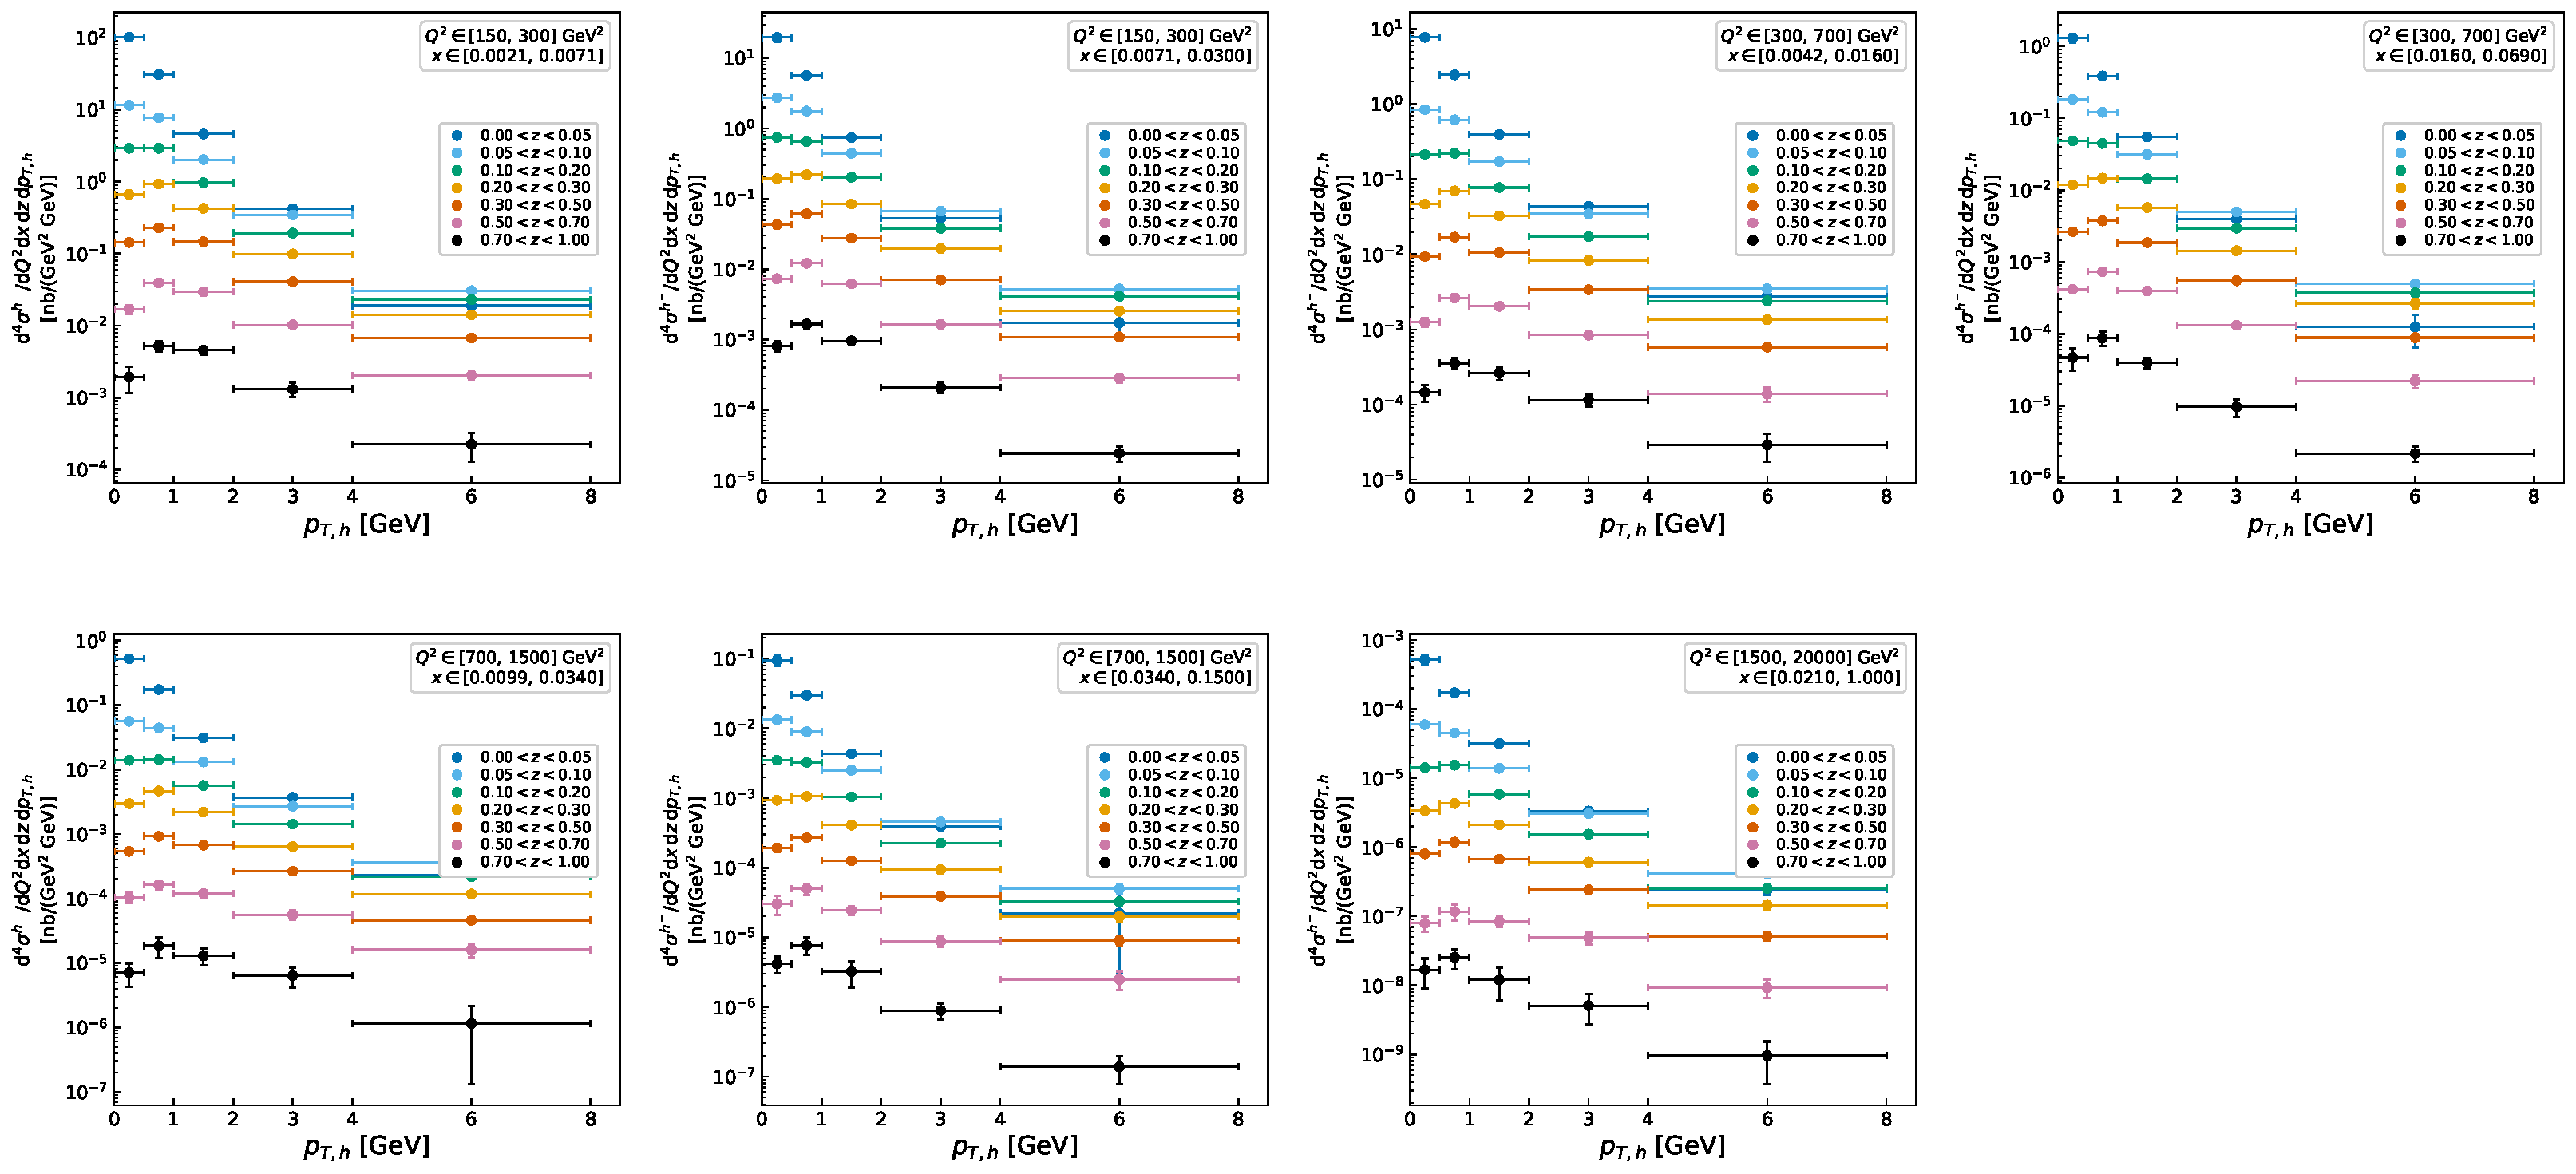
\includegraphics[width=0.98\textwidth,height=0.82\textheight,keepaspectratio]{figures/fig_results_xsec_density_born_cone_env100_7panel_hminus_z005_20261019.pdf}
  \caption{Born-level provisional cross-section density for $\hminus$
  from the iterative Bayesian unfolding, plotted as
  $\mathrm{d}^{4}\sigma/(\mathrm{d}\Qsq\,\mathrm{d}x\,
  \mathrm{d}z\,\mathrm{d}\pTh)$ in $\mathrm{nb}\,\GeV^{-3}$, at
  $\mathcal{L}_{\mathrm{data}}=351000.0~\mathrm{nb}^{-1}$.
  $C_{\mathrm{rad}}$ is applied per-bin post-unfold from the DJANGOH14
  (xFGen$<$0, EMPZ$>$45) table.  The points are the background-subtracted
  Born-level values of the superseded 2026-10-15 clean-release basis, which
  predates the OPT-A baseline promotion: the electron, V0, and low-$\Qsq$
  backgrounds are subtracted from the data vector before unfolding.  The band
  shows the quoted total systematic uncertainty of the frozen 2026-10-19
  budget, superseded as a quoting basis, whose median totals are
  $7.320288331169215\%$ for $\hplus$ and
  $7.637124635311324\%$ for $\hminus$.  This Born-level provisional figure
  carries internal-review status and is not physics-final.  Produced from the
  dated 2026-10-19 cross-section package
  \texttt{plots/cross\_sections/cone\_born\_7panel\_env100\_xcap\_2026-10-19/}.}
  \label{fig:results:release351-cone-xsec-density-hminus}
\end{figure}

\begin{figure}[p]
  \centering
  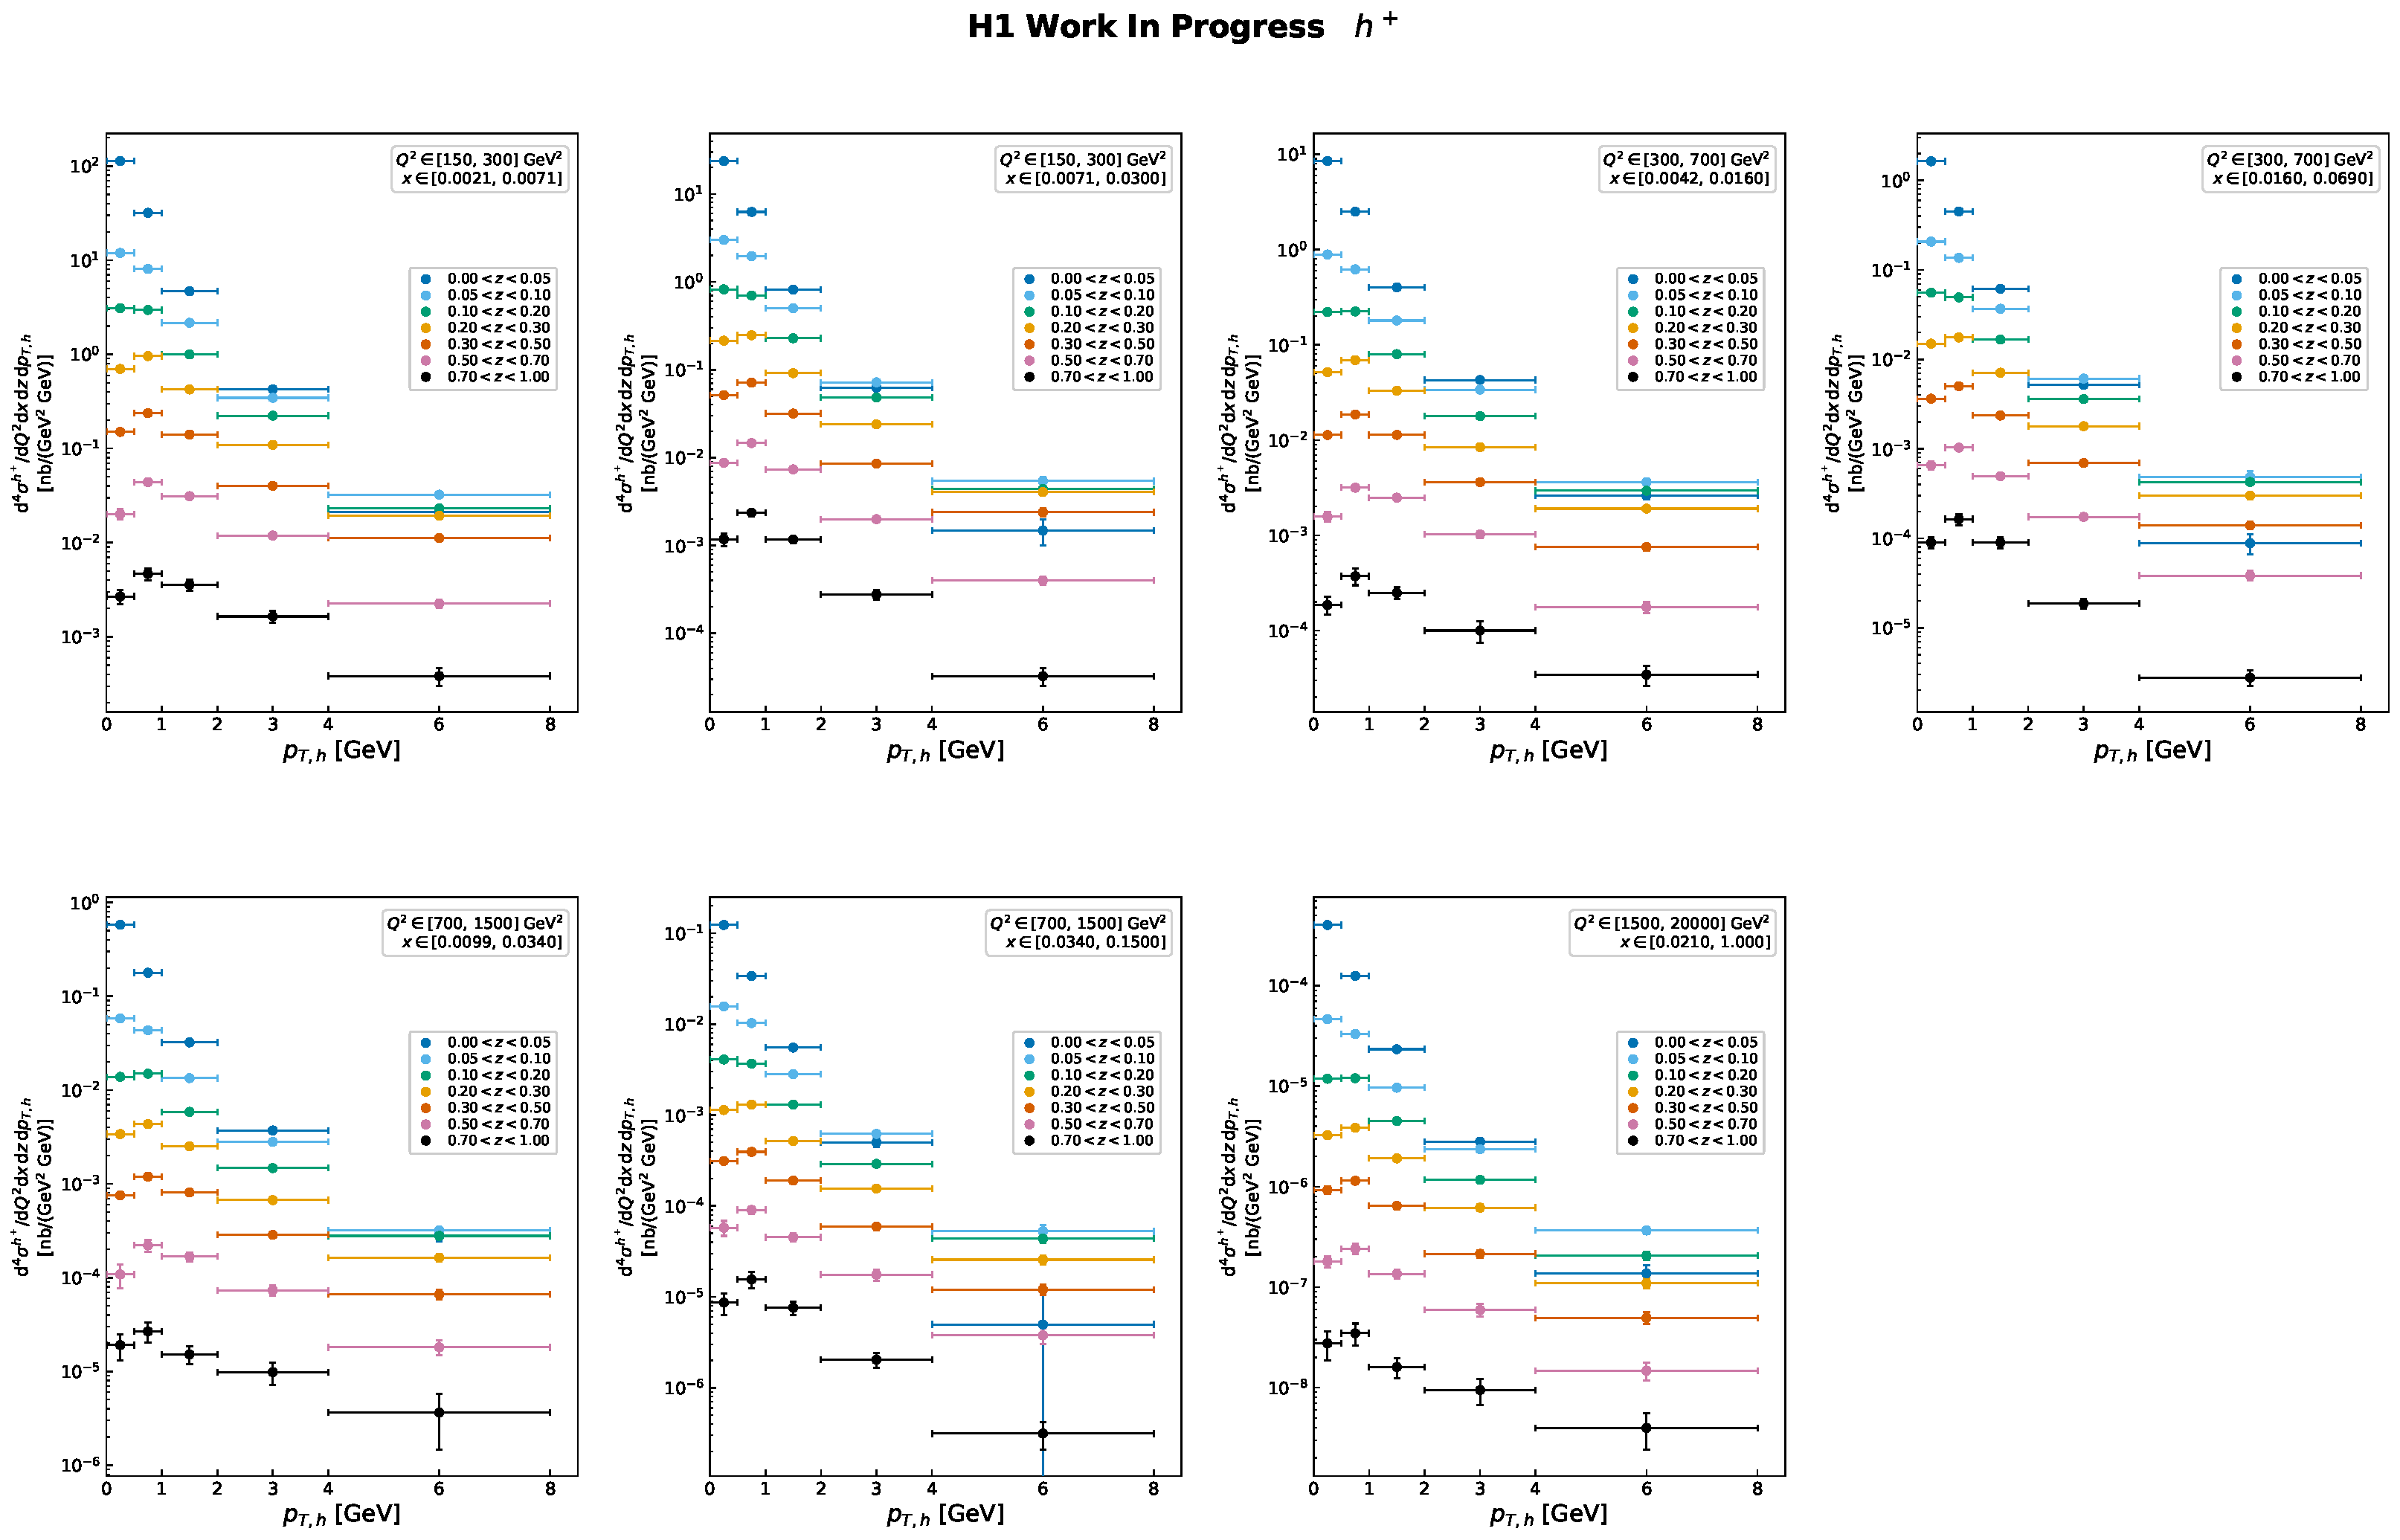
\includegraphics[width=0.98\textwidth,height=0.82\textheight,keepaspectratio]{figures/fig_results_xsec_density_born_crad13_coherentprior_7panel_hplus_z005_20261008.pdf}
  \caption{Born-level provisional cross-section density for $\hplus$ from the
  iterative Bayesian unfolding, on the superseded xFcut basis that predates
  the detector-interaction correction (2026-10-08 rendering), plotted as
  $\mathrm{d}^{4}\sigma/(\mathrm{d}\Qsq\,\mathrm{d}x\,
  \mathrm{d}z\,\mathrm{d}\pTh)$ in $\mathrm{nb}\,\GeV^{-3}$, with the
  response matrix's own generator-level distribution as the unfolding prior at
  $\mathcal{L}_{\mathrm{data}}=351000.0~\mathrm{nb}^{-1}$.
  $C_{\mathrm{rad}}$ is applied per-bin post-unfold from the DJANGOH14 xFcut
  (xFGen$<$0, EMPZ$>$45) table, and the vertical error bars show the full
  13-component systematic total, including the radiative components
  \texttt{c\_rad\_gen\_rel} and \texttt{c\_rad\_stat\_rel}.  The plot uses the
  canonical $|\eta_h|<1.6$ selection, with background handling by response
  fake-fraction subtraction only.  These values, which predate the
  detector-interaction correction, are superseded by the current cone-based
  figures above and are not physics-final.}
  \label{fig:results:release351-expanded-xsec-density-hplus}
\end{figure}

\begin{figure}[p]
  \centering
  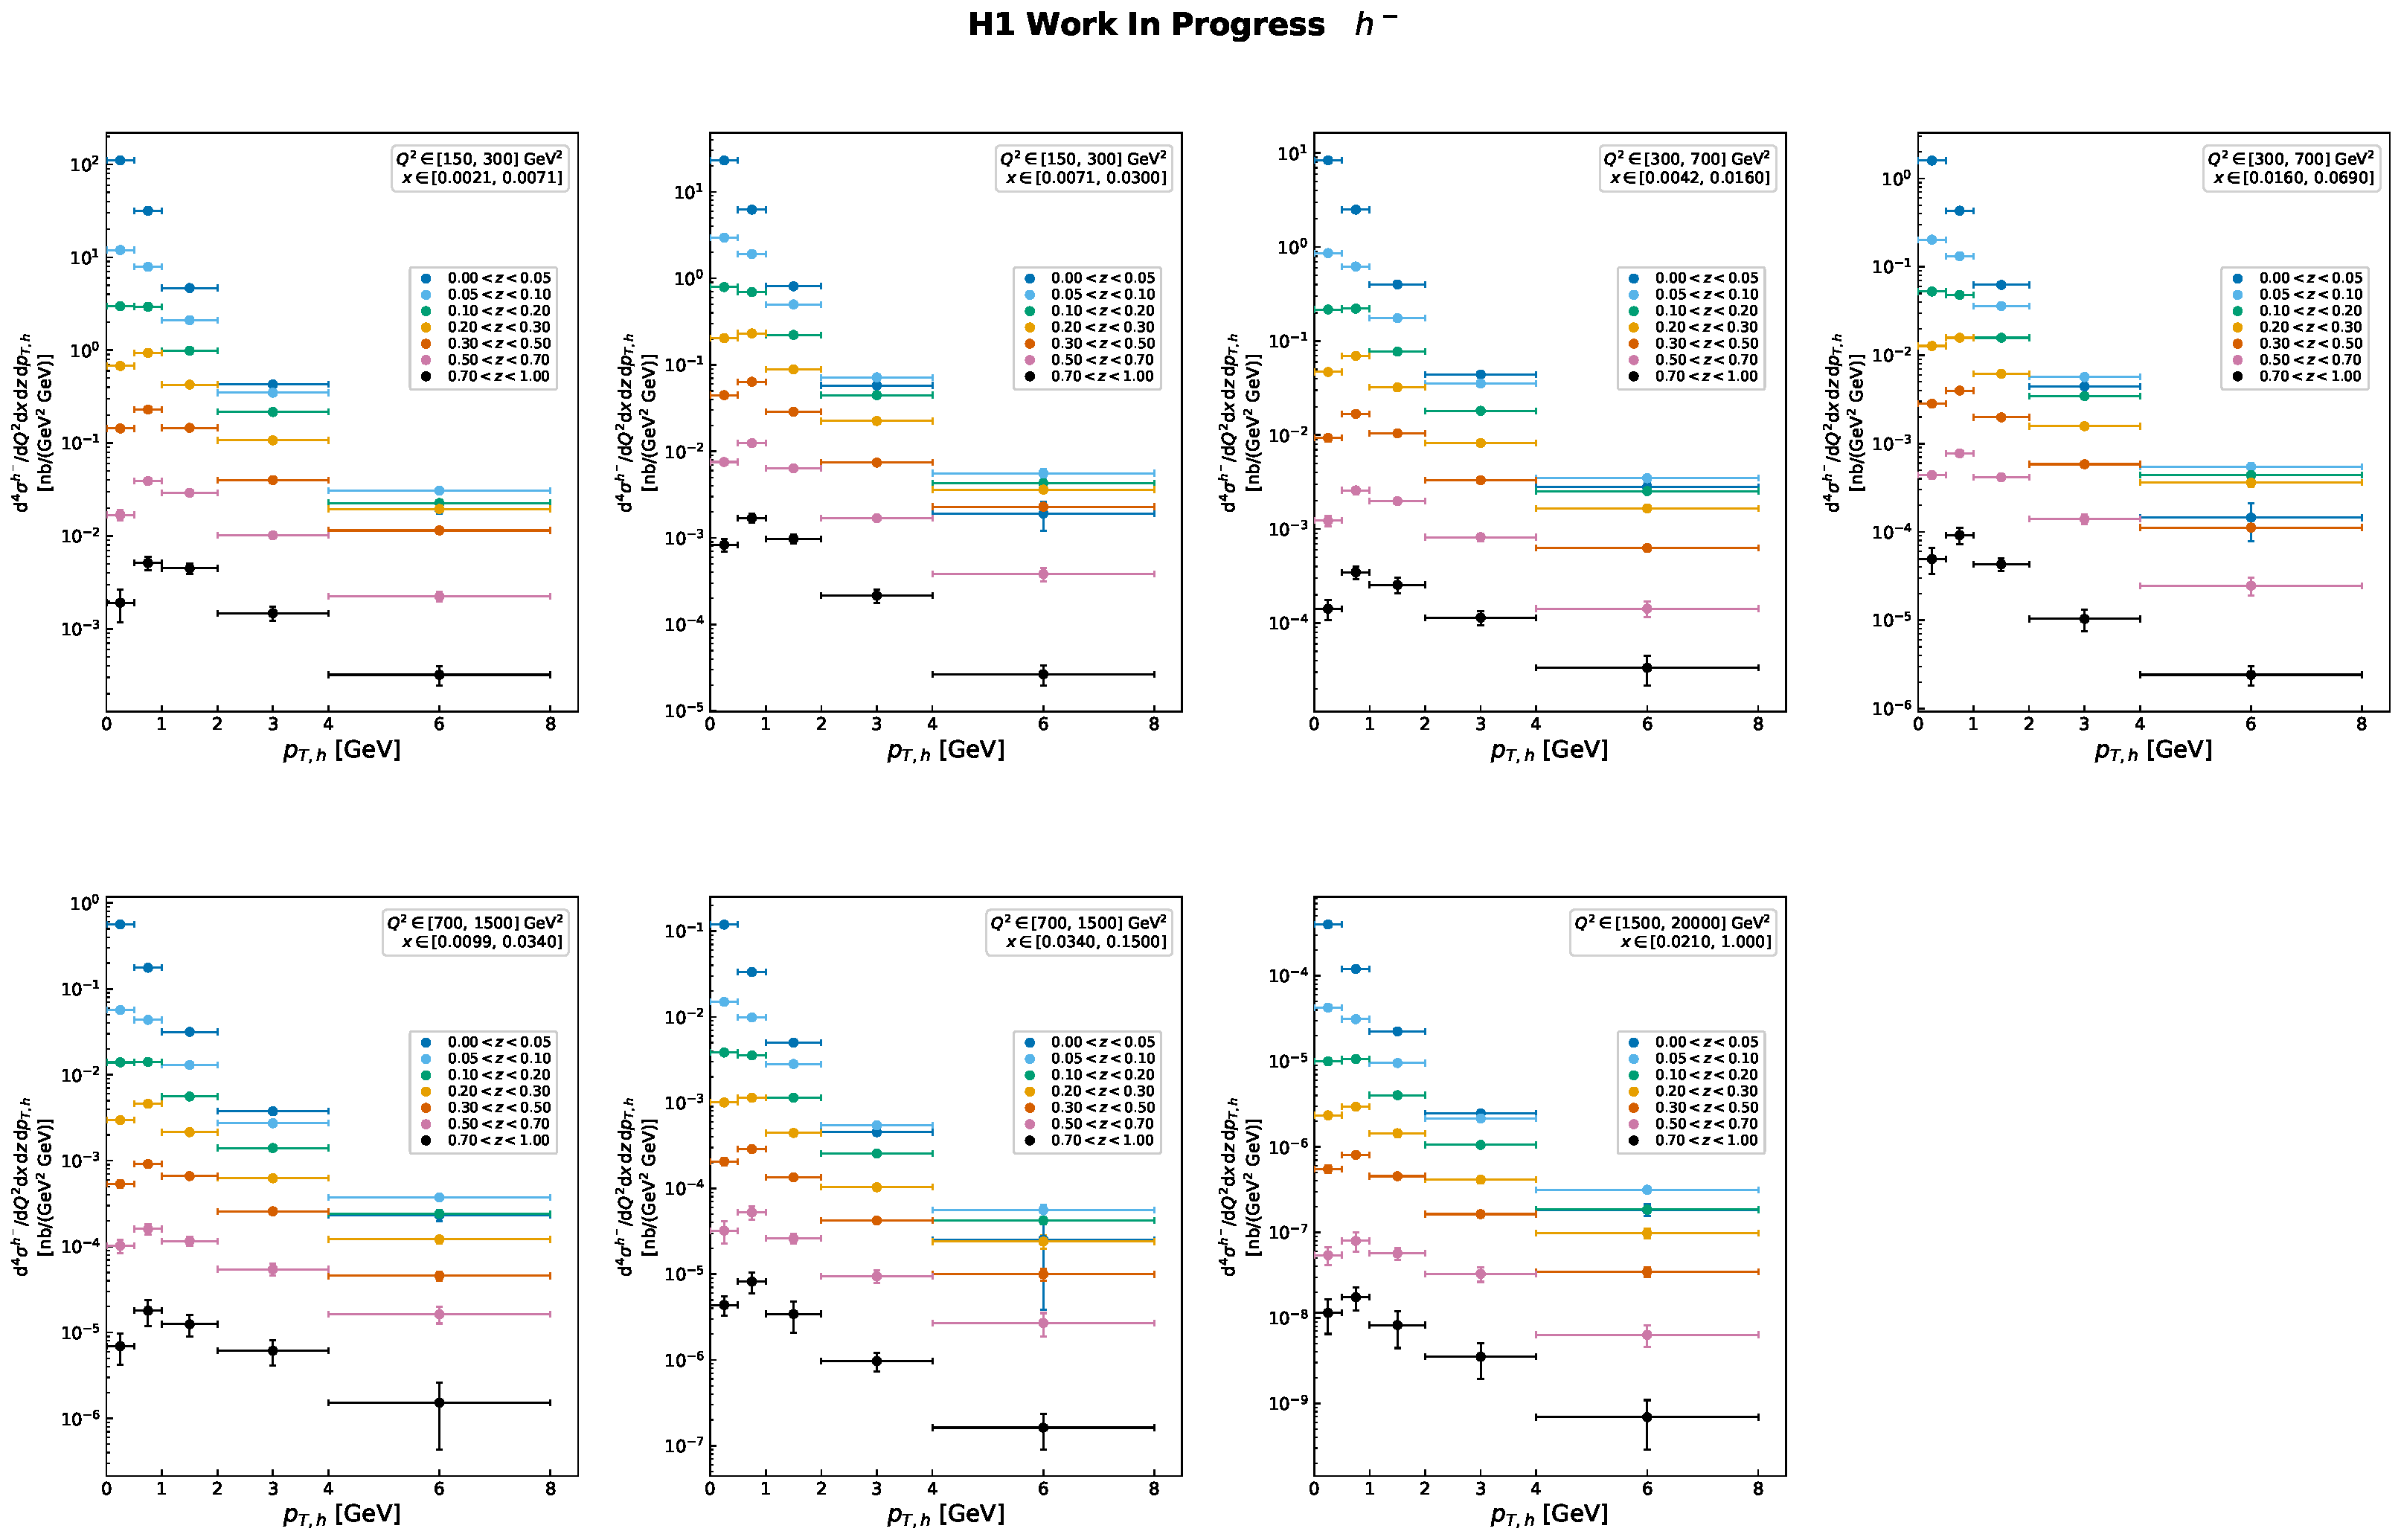
\includegraphics[width=0.98\textwidth,height=0.82\textheight,keepaspectratio]{figures/fig_results_xsec_density_born_crad13_coherentprior_7panel_hminus_z005_20261008.pdf}
  \caption{Born-level provisional cross-section density for $\hminus$ from the
  iterative Bayesian unfolding, on the superseded xFcut basis that predates
  the detector-interaction correction (2026-10-08 rendering), plotted as
  $\mathrm{d}^{4}\sigma/(\mathrm{d}\Qsq\,\mathrm{d}x\,
  \mathrm{d}z\,\mathrm{d}\pTh)$ in $\mathrm{nb}\,\GeV^{-3}$, with the
  response matrix's own generator-level distribution as the unfolding prior at
  $\mathcal{L}_{\mathrm{data}}=351000.0~\mathrm{nb}^{-1}$.
  $C_{\mathrm{rad}}$ is applied per-bin post-unfold from the DJANGOH14 xFcut
  (xFGen$<$0, EMPZ$>$45) table, and the vertical error bars show the full
  13-component systematic total, including the radiative components
  \texttt{c\_rad\_gen\_rel} and \texttt{c\_rad\_stat\_rel}.  The plot uses the
  canonical $|\eta_h|<1.6$ selection, with background handling by response
  fake-fraction subtraction only.  These values, which predate the
  detector-interaction correction, are superseded by the current cone-based
  figures above and are not physics-final.}
  \label{fig:results:release351-expanded-xsec-density-hminus}
\end{figure}

\subsection{Interpretation of Present Tables}
\label{sec:results:present-tables}

The release tables are suitable for validating the detector correction,
unfolding implementation, binning, and already-derived systematic components.
They are not yet the final multiplicity tables: the cross section now has the
per-bin post-unfold $C_{\mathrm{rad}}$ applied, with its uncertainty carried
as the radiative generator-difference and radiative-statistics components,
but no corrected inclusive DIS denominator is
available, so the multiplicity mapping remains pending. In particular, a
cross-section-ratio radiative diagnostic is not a substitute for the required
$M_{\mathrm{norad}}/M_{\mathrm{rad}}$ mapping.  The appendix tables of this
note are rendered on the current background-subtracted basis; their basis
statement is given in App.~\ref{app:born-xsec-tables}.

The release should therefore be circulated externally with the following status
qualification: detector, unfolding, background-subtraction, luminosity, and
radiative uncertainties are included, the radiative ones as the
generator-difference and statistical components; the five detector components
are full-chain single-sided shifts, with the HFS legs produced in the plus
direction only and their sign symmetry assumed, and the tracking-efficiency
component remains a data-side conservative shift; the electron, V0, and
low-$\Qsq$ backgrounds are subtracted before unfolding while the
detector-interaction class is removed response-internally, and the applied
$C_{\mathrm{rad}}$ is mixed-beam only; and the cut
variations are robustness checks rather than central results.  The frozen
systematic editions are superseded as a quoting basis and the budget is being
regenerated on the OPT-A nominal, so no per-bin uncertainty or total is final
until the regenerated budget passes review
(Sec.~\ref{sec:syst:budget-regeneration}).  No PID-separated
pion, kaon, or proton result is provided.

\subsection{Low-$\Qsq$ Companion Status}
\label{sec:results:lowq2-companion}

The low-$\Qsq$ charged-SIDIS analysis is a separate companion analysis covering
$5<\Qsq<100~\GeVsq$.  Its current publication-track headline is preliminary:
$\sigma_{\mathrm{total}}=463.9\pm5~\mathrm{(stat)}\pm47.9~\mathrm{(syst)}~\mathrm{nb}$
on the all-768-cell v3p3p1 TUnfold treatment, with $\sigma(\hplus)=233.3~\mathrm{nb}$,
$\sigma(\hminus)=230.7~\mathrm{nb}$, $\hplus/\hminus=1.011$, and
$\Ah=+0.00566$.  The low-$\Qsq$ result remains preliminary because several
systematic follow-ups are open, including validation of shifted-MC reuse at the
v3p3 fiducial, replacement of the analytic statistical quote by the bootstrap
value where appropriate, and additional checks of source summaries and
regularization details.  These low-$\Qsq$ numbers are not inputs to the
high-$\Qsq$ release.

% End of Results section.
